\documentclass{article}
\usepackage{subcaption} % For subfigures
\usepackage{graphicx}   % For including images

\begin{document}

\begin{figure}[h]
    \centering
    \begin{subfigure}{0.45\textwidth}
        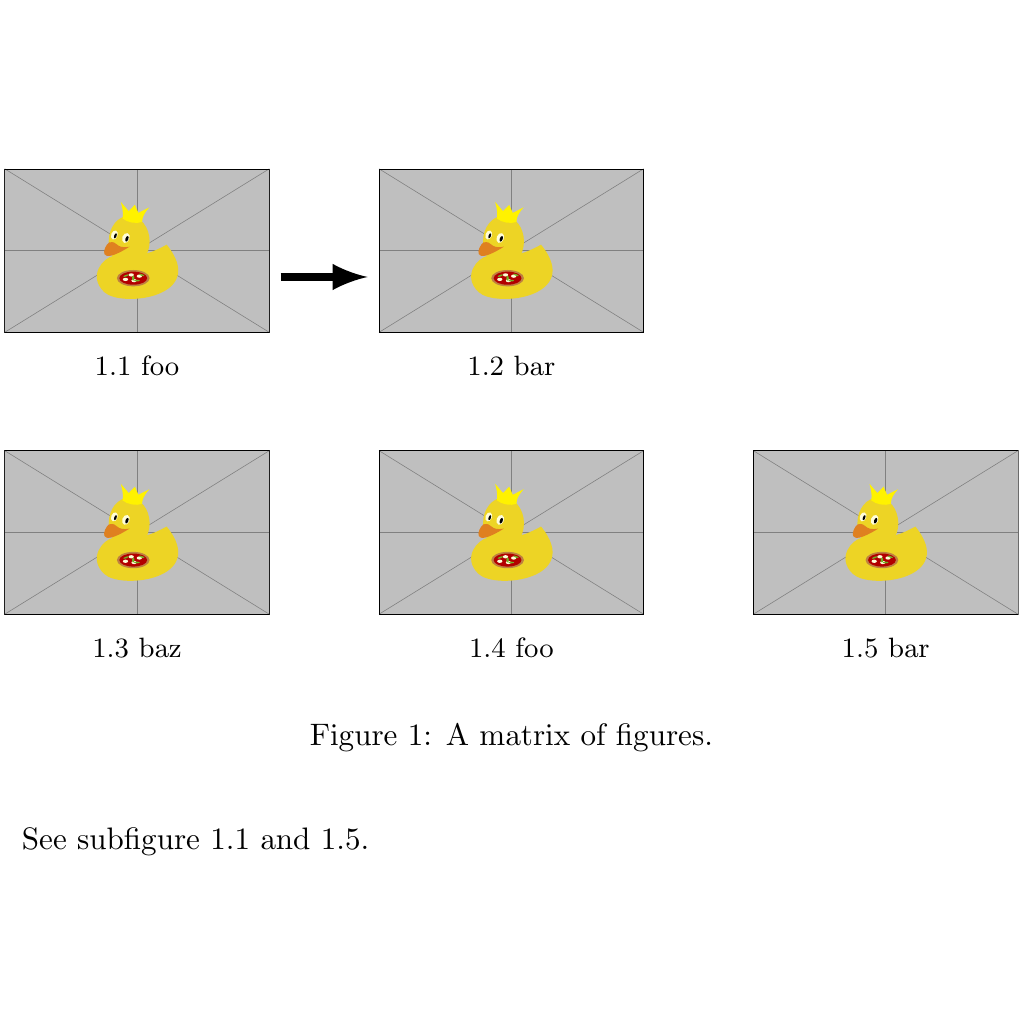
\includegraphics[width=\linewidth]{sample_201.png}
        \caption{foo}
        \label{fig:sub1}
    \end{subfigure}
    \hfill
    \begin{subfigure}{0.45\textwidth}
        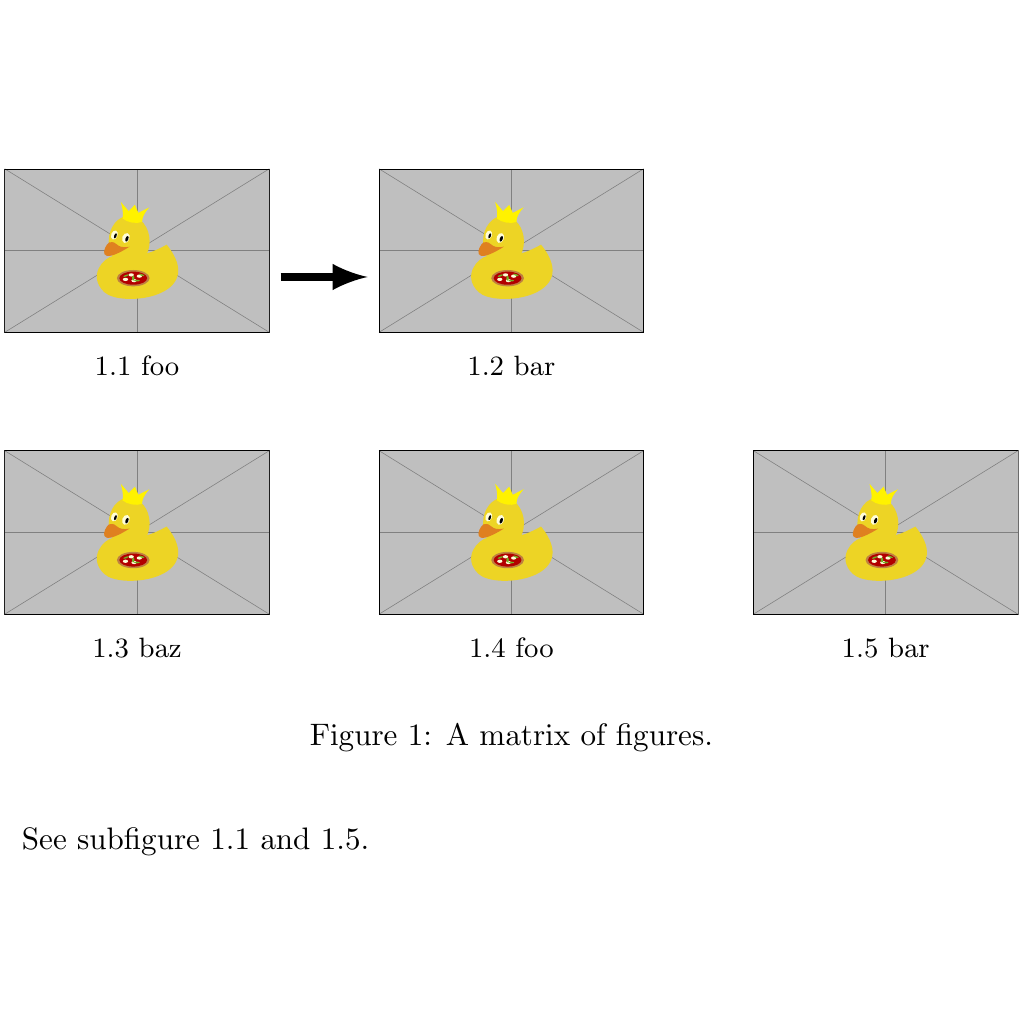
\includegraphics[width=\linewidth]{sample_201.png}
        \caption{bar}
        \label{fig:sub2}
    \end{subfigure}
    
    \begin{subfigure}{0.45\textwidth}
        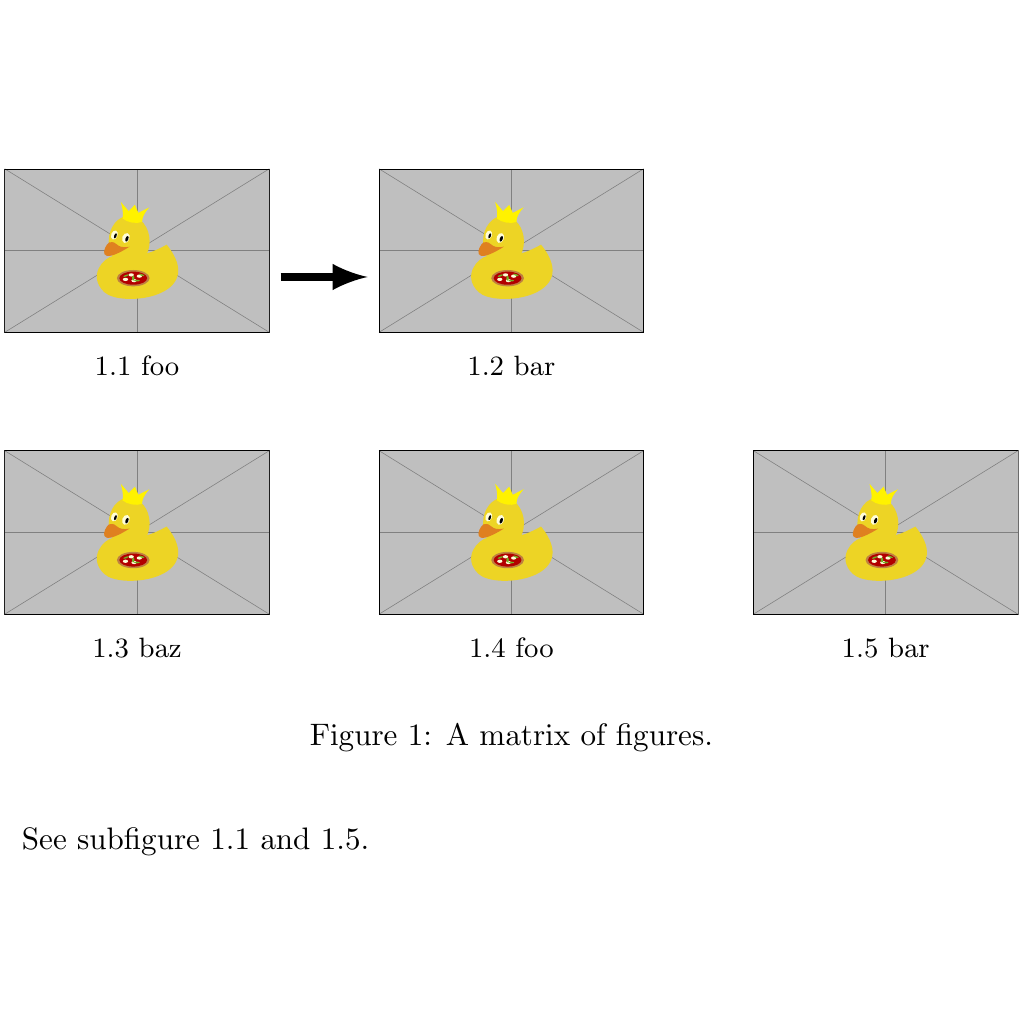
\includegraphics[width=\linewidth]{sample_201.png}
        \caption{baz}
        \label{fig:sub3}
    \end{subfigure}
    \hfill
    \begin{subfigure}{0.45\textwidth}
        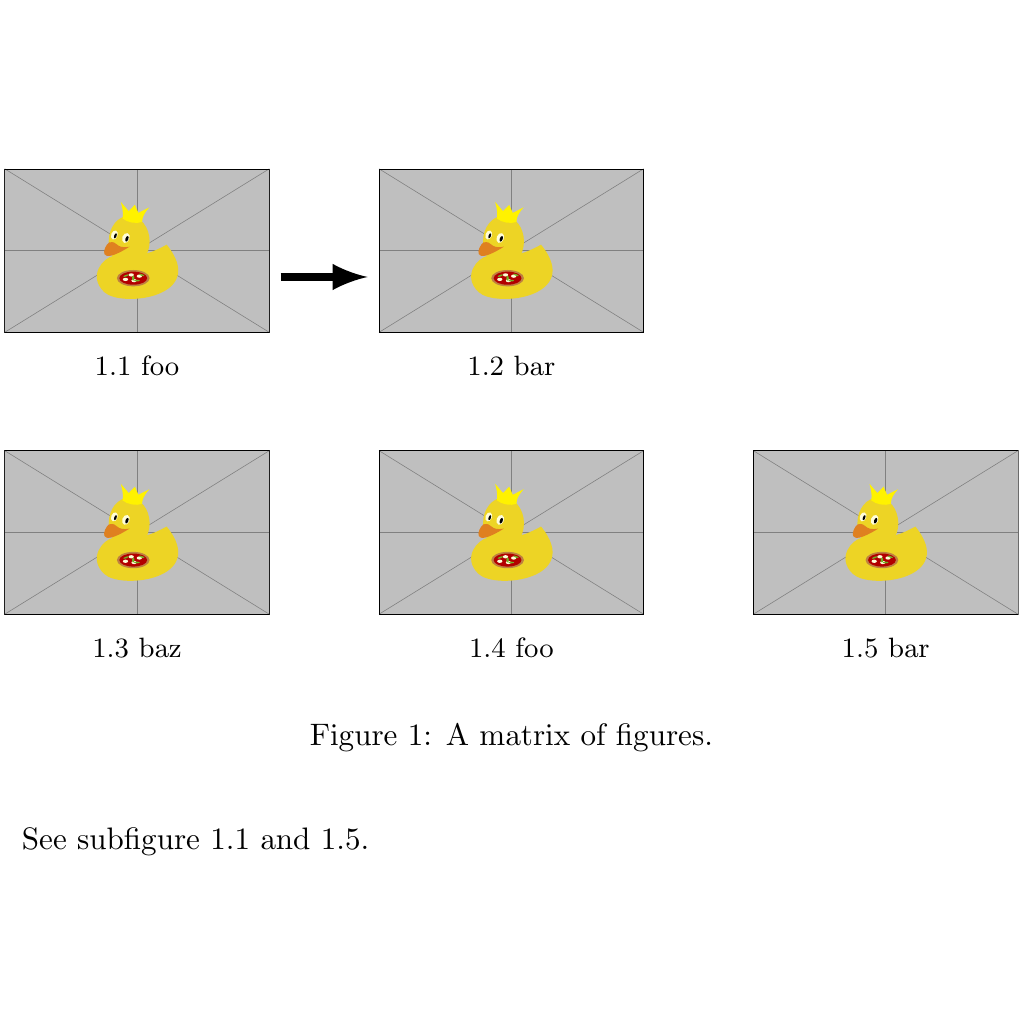
\includegraphics[width=\linewidth]{sample_201.png}
        \caption{foo}
        \label{fig:sub4}
    \end{subfigure}
    \hfill
    \begin{subfigure}{0.45\textwidth}
        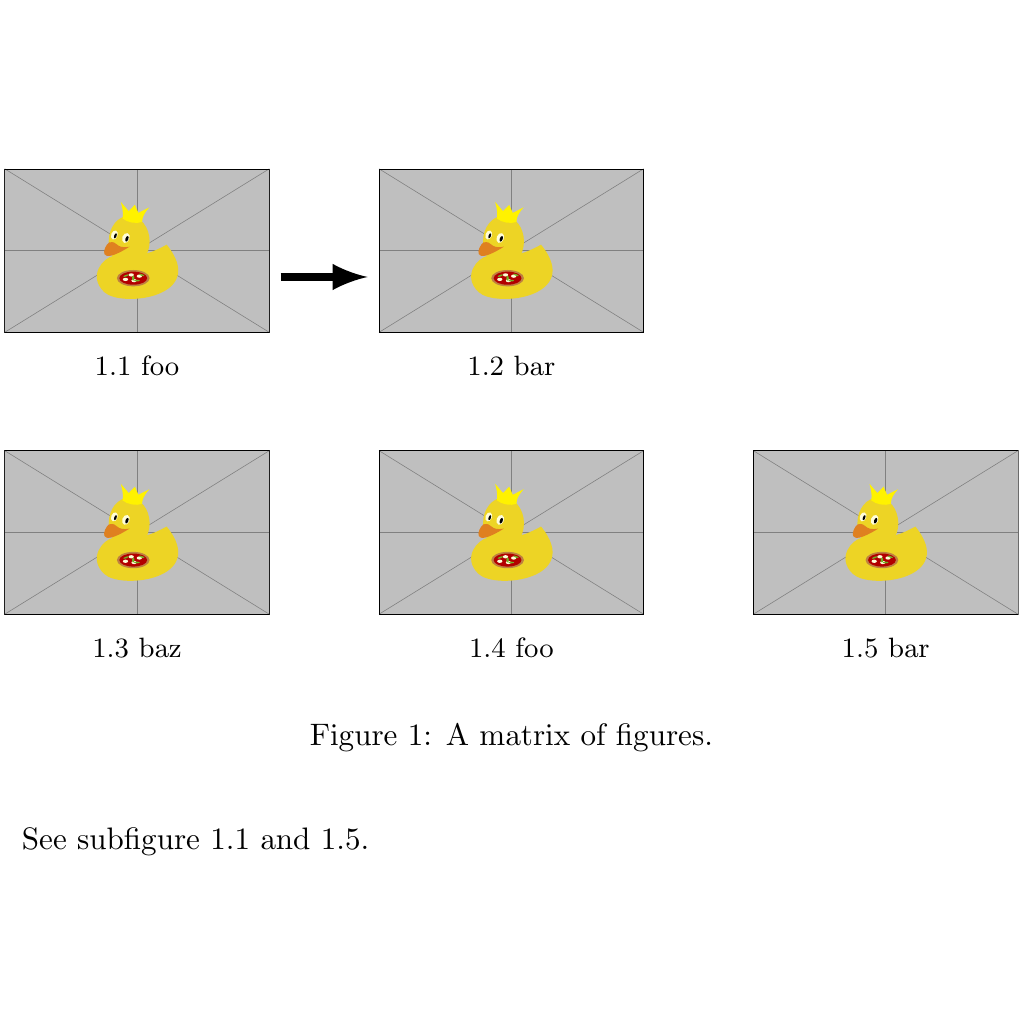
\includegraphics[width=\linewidth]{sample_201.png}
        \caption{bar}
        \label{fig:sub5}
    \end{subfigure}
    
    \caption{A matrix of figures.}
    \label{fig:matrix}
\end{figure}

See subfigure \ref{fig:sub1} and \ref{fig:sub5}.

\end{document}